\documentclass[fr,license=none]{../../../eplsummary}

\usepackage{../../../eplunits}
\usepackage{../../../eplelec}
\usepackage{circuitikz}
\sisetup{detect-all}

\makeatletter
\providecommand\add@text{}
\renewcommand\u[1]{%
  \gdef\add@text{[\si{#1}\gdef\add@text{}]}}% 
\renewcommand\tagform@[1]{%
  \maketag@@@{\llap{\add@text\quad}(\ignorespaces#1\unskip\@@italiccorr)}%
}
\makeatother

\hypertitle[']{électromagnétisme appliqué}{5}{ELEC}{1350}
{Gaetan Cassiers\and Antoine Paris\and Philippe Verbist}
{Christophe Craeye et Danielle Janvier}

% TODO
% - utiliser les nouvelles commandes partout
% - changer les 'r' dans les formules de champs/potentiels
% d'une distribution de charge en vecteur
% - + liste des TODOs dans la synthèse

\part{\'{E}lectrostatique}
\section{Loi de Coulomb et champ électrique}
\subsection{Loi de Coulomb}
\begin{mylaw}
La loi de Coulomb est une loi expérimentale qui
décrit la force d'attraction (ou de répulsion)
entre deux charges
\begin{equation}
	\vec{F} = \frac{q_1q_2}{4\pi\perm_0r^2}\hat{a}_r.
	\u{\newton}
\end{equation}

Cette force agit sur la ligne joignant les deux charges
et est répulsive si les charges sont
de même signe, attractive dans le cas contraire.
\end{mylaw}

\subsection{Champ électrique}
\begin{mydef}
Le champ électrique subi par une charge $q$
est défini comme la force électrique subie
par unité de charge
\begin{equation}
	\E \eqdef \frac{\vec{F}}{q}.
	\u{\newton\per\coulomb}
	\label{eq:electric-field}
\end{equation}
\end{mydef}

\subsubsection{D'une seule charge}
\begin{equation}
	\E = \frac{q}{4\pi\perm_0r^2}\hat{a}_r.
\end{equation}

\begin{myprop}
Le champ électrique étant une fonction linéaire
de la charge, le principe de superposition s'
applique.
\end{myprop}

\subsubsection{D'une distribution de charge}
Pour une distribution de charge (linéique, de surface
ou de volume), on a
\begin{equation}
	Q = \int_{\text{vol}} \rho_v\dif v.
	\u{\coulomb}
\end{equation}

En définissant un référentiel quelconque comme
sur la figure \ref{fig:referentiel}, on peut
écrire $\vec{E}$ de manière tout à fait générale
\begin{equation}
	\vec{E}(r) = \int_{\text{vol}} \frac{\rho_v(r')\dif v}{4\pi\perm_0|r-r'|^2}
	\frac{\overrightarrow{r - r'}}{|r - r'|}.
\end{equation}

\begin{figure}
	\centering
	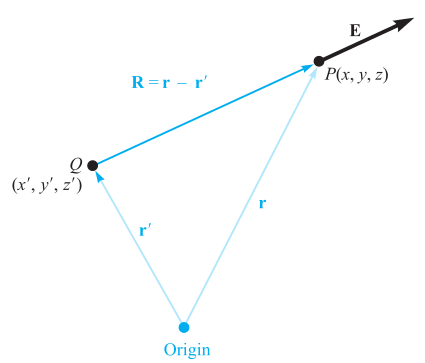
\includegraphics[scale=0.5]{img/referentiel.png}
	\caption{Référentiel quelconque.}
	\label{fig:referentiel}
\end{figure}

\section{Densité de flux électrique, loi de Gauss et divergence}
\subsection{Champ de déplacement électrique}
Le champ de déplacement électrique ou densité de flux
électrique est donné par
\begin{equation}
	\D = \perm \E.
	\u{\coulomb\per\meter\squared}
	\label{eq:def-d}
\end{equation}

\subsection{Loi de Gauss}
\begin{mylaw}
Le flux électrique à travers une surface
fermée est égal à la quantité de charge située à
l'intérieur de cette surface fermée.
\end{mylaw}

Mathématiquement,
\begin{equation}
	\oint_\text{S} \vec{D}_\text{S} \cdot \dif \vec{S} 
	= \int_\text{vol} \rho_v \dif v = Q
	\label{eq:gauss}
\end{equation}

où $\vec{S}$ est défini comme sortant de la surface. 

La loi de Gauss permet de calculer des champs électriques
pour des distributions de charges symétriques.

On peut aussi écrire cette équation sous la forme
\begin{equation}
	\divn \D = \rho_v
	\label{eq:gauss-dif}
\end{equation}

en se rappelant de la définition de la divergence.

\begin{mydef}
La divergence d'un vecteur de densité de
flux est égal au flux sortant d'une petit surface
fermée par unité de volume lorsque ce volume tend
vers zéro.
\end{mydef}

Une divergence positive indique donc la présence d'une
\textit{source} tandis qu'une divergence négative indique
la présence d'un \textit{puits}.

On peut passer d'une équation à l'autre en utilisant
le théorème de la divergence
\begin{equation}
	\oint_\text{S} \vec{D}_\text{S} \cdot \dif \vec{S}
	= \int_\text{vol} \divn \D \dif v.
\end{equation}

\section{\'{E}nergie et potentiel}
\subsection{Potentiel}
Supposons que l'on veuille déplacer une charge $Q$ d'une
distance $\dif \vec{l}$ dans un champ électrique $\E$.
Par \ref{eq:electric-field}, la force sur cette charge
est
\[ \vec{F}_E = Q\E. \]

La composante de cette force dans la direction
$\dif \vec{l}$ est donc
\[ \vec{F}_{EL} = \vec{F}_E \cdot \hat{a}_l = Q\E\cdot \hat{a}_l. \]

Pour vaincre cette force et déplacer la charge, il
faut appliquer une force
\[ \vec{F}_{appl} = -Q\E \cdot \hat{a}_l. \]

Le travail effectué par une source externe pour
déplacer cette charge d'une distance $\dif l$ est
donc
\[ \dif W = -Q\E \cdot \hat{a}_l \dif l = -Q\E \cdot \dif \vec{l} \]

et le travail total pour déplacer une charge d'un
point $A$ à un point $B$ est donné par
\[ W = -Q \int_A^B \E \cdot \dif \vec{l}. \]

\begin{mydef}
On définit ensuite la \textit{différence de potentiel} $V$
comme le travail effectué (par une source externe) pour
déplacer une charge unitaire positive d'un point à un
autre dans un champ électrique
\begin{equation}
	\Delta V = V_B - V_A = -\int_A^B \E \cdot \dif \vec{l}.
	\u{\volt}
	\label{eq:potdef}
\end{equation}
\end{mydef}

Lorsqu'on utilise cette équation, on est souvent amené
à définir une référence de potentiel nul. En général, on
utilise pour cela soit un point de référence représentant
la \textit{terre} soit un point situé à une distance
\textit{infinie} du problème.

\begin{mydef}
Une \textit{surface équipotentielle} est une surface
composée de tous les points ayant le même potentiel.
Toutes les lignes de champ électrique sont perpendiculaires
à cette surface aux points d'intersections. Aucun travail
n'est donc nécessaire pour déplacer une charge sur une
surface équipotentielle.
\end{mydef}

\begin{myprop}
Aucun travail n'est effectué pour déplacer une charge
le long d'un chemin fermé
\begin{equation}
	\oint \E \cdot \dif l = 0.
	\label{eq:E-conservatif}
\end{equation}
Cette équation est valide pour les champs \textit{statique}.
On dit dans ce cas que $\E$ est un champ \textit{conservatif}.
On peut réecrire cette équation comme ceci
\begin{equation}
	\rotn \E = 0
	\label{eq:E-conservatif-dif}
\end{equation}
en utilisant les théorèmes intégraux.
\end{myprop}

Par conséquent, le champ $\E$ dérive d'un potentiel
\begin{equation}
	\E = - \gradn V.
	\label{eq:e-grad-v}
\end{equation}
Cette équation nous permet d'obtenir un peu d'intuition
sur le champ électrique :
\begin{enumerate}
	\item La norme du champ électrique est donnée par la
	valeur maximum de la dérive du potentiel par rapport à la
	distance ;
	\item La direction du champ électrique est opposée
	à la direction dans laquelle le potentiel augmente
	le plus rapidement.
\end{enumerate}

\subsubsection{Potentiel d'une charge ponctuelle}
\begin{equation}
	V = \frac{Q}{4\pi\perm_0}.
	\label{eq:pot-charge}
\end{equation}

\subsubsection{Potentiel d'une distribution de charges}
En utilisant à nouveau le référentiel de la figure
\ref{fig:referentiel}
\begin{equation}
	V(r) = \int_{vol} \frac{\rho_v(r')}{4\pi\perm_0
	|r-r'|}\dV'.
	\label{eq:elec-pot}
\end{equation}

\subsection{Dipôle électrique}
\begin{mydef}
Un dipôle électrique est composé de deux charges ponctuelles
de normes égales mais de signe opposé séparé par une distance
faible par rapport à la distance à laquelle on veut calculer
le champ électrique.
\end{mydef}

\begin{mydef}
On définit le moment du dipole
\begin{equation}
	\vec{p} = Q\vec{d}
	\u{\coulomb\meter}
\end{equation}
où $Q$ est la charge positive du dipôle, et $\vec{d}$
le vecteur pointant de la charge négative vers la charge
positive.
\end{mydef}

Pour trouver le champ électrique et le potentiel électrique
d'un dipôle, on commence par trouver le potentiel dû aux
deux charges via \ref{eq:pot-charge} et on utilise
ensuite l'approximation de Fraunhofer (comme en physique 3
pour les ondes) pour trouver ce même potentiel à une
grande distance du dipôle. On utilise ensuite l'équation
\ref{eq:e-grad-v} pour trouver le champ électrique.
C'est une bonne illustration de comment utiliser le
potentiel pour simplifier les calculs. De plus, cela
justifie la méthode des images (voir sous-section
\ref{subseq:images}).

\subsection{Dénsité d'énergie}
\begin{equation}
	W_E = \frac{1}{2} \int_{vol} \D \cdot \E \dif v
	= \frac{1}{2} \int_{vol} \perm_0\E^2 \dif v.
\end{equation}

\section{Conducteurs et diélectriques}
\subsection{Courant et densité de courant}
\begin{mydef}
Un mouvement de charge constitue un \textit{courant}
\begin{equation}
	I \eqdef \fdif{Q}{t}.
	\u{\ampere}
	\label{eq:current}
\end{equation}
Le courant est donc défini comme un mouvement de charge
positive.
\end{mydef}

\begin{mydef}
La densité de courant est définie par
\begin{equation}
	\J \eqdef \frac{\Delta I}{\Delta S} \hat{\mu}_n
	\u{\ampere\per\meter\squared}
	\label{eq:current-density}
\end{equation}
où $\hat{\mu}_n$ est normal à $\Delta S$ dans la
direction du courant. On peut donc réecrire
le courant comme
\begin{equation}
	I = \int_S \J \cdot \dif \vec{S}.
\end{equation}

% A CONFIRMER (même si ça semble relativement logique)
\begin{myrem}
Attention : alors qu'on définissait $\dif \vec{S}$ comme
sortant de la surface pour la Loi de Gauss, ici $\dif \vec{S}$
est défini dans le sens du courant.
\end{myrem}

\begin{myrem}
Imaginons qu'un courant circule dans une feuille d'épaisseur
infinitisémale, dans ce cas, $\J$ est infini. On définit
dans ce cas la densité de courant surfacique $\K [\si{\ampere
\per\meter}]$ comme illustré sur la figure \ref{fig:current-surface-density}. Si $\K$ est uniforme, on a
\begin{equation}
	I = Kb
\end{equation}
où $b$ est mesuré perpendiculaire à la direction du courant.
Si $\K$ n'est pas uniforme, on a cette fois
\begin{equation}
	I = \int K \dif N
\end{equation}
où $\dif N$ est un élément infinitisémal du chemin par lequel
circule le courant.
\end{myrem}

\begin{figure}[ht]
	\centering
	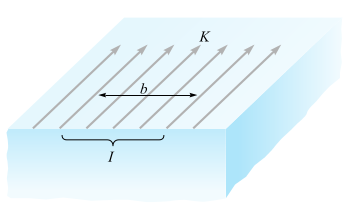
\includegraphics[scale=0.5]{img/current-surface-density.png}
	\caption{Illustration de la densité de courant
	surfacique $\K$.}
	\label{fig:current-surface-density}
\end{figure}

\end{mydef}
A partir de l'équation \ref{eq:current}, on peut écrire
\[ \Delta I = \frac{\Delta Q}{\Delta t} = \rho_v\Delta S
\frac{\Delta x}{\Delta t} = \rho_v\Delta S v_x \]
et donc via \ref{eq:current-density}
\begin{equation}
	\J = \rho_v\vec{v}
	\label{eq:convection}
\end{equation}
ce qui montre bien qu'un mouvement de charge constitue
un courant. Ce type de courant s'appelle un \textit{courant
de convection}.

\subsection{Continuité du courant}
\begin{mylaw}[Conservation de la charge]
Une charge électrique ne peut ni être créée ni détruite.
\end{mylaw}

De ce principe de conservation de la charge,
on peut écrire
\begin{equation}
	I = \oint_S \J \cdot \dif S = - \fdif{Q_i}{t}
\end{equation}
où $Q_i$ représente la charge située dans la
surface fermée.

En utilisant le théorème de la divergence, on
peut à nouveau réécrire cette équation sous forme
différentielle
\begin{equation}
	\divn \J = - \fpart{\rho_v}{t}.
	\label{eq:cont-cur-dif}
\end{equation}

\subsection{Conducteur métallique}
Dans un conducteur métallique, les électrons ont
une vitesse moyenne qu'on appelle la vitesse de
dérive $\vec{v}_d$. Les cours de dispositifs nous
montre que
\begin{equation}
	\vec{v}_d = -\mu_e\E
	\label{eq:driftv}
\end{equation}
où $\mu_e$ est le mobilité des électrons mesurées
en \si{\meter\squared\per\volt\per\second}. En injectant
\ref{eq:driftv} dans \ref{eq:convection} on obtient
\begin{equation}
	\J = -\rho_e\mu_e\E
\end{equation}
où $\rho_e$ est la densité des charges des électrons (et
donc est négatif). On définit la \textbf{conductivité}
\begin{equation}
	\sigma = -\rho_e\mu_e
	\u{\siemens\per\meter}
\end{equation}
telle que
\begin{equation}
	\J = \sigma \E
\end{equation}
et la résistivité $\rho = \sigma^{-1}$ mesurée
cette fois en \si{\ohm\meter}.

\begin{myrem}
Cette dernière équation couplé à l'équation de
continuité du courant \ref{eq:cont-cur-dif} dans
un cas statique
\begin{equation}
	\divn (\sigma \E) = 0
\end{equation}
permet parfois d'obtenir des informations sur
$\E$ lorsque l'injection de l'ansatz dans les
équations de Maxwell ne donne rien\footnote{C'est
le cas par exemple si \ref{eq:E-conservatif-dif}
donne $0 = 0$ et si $\rho_v$ dans \ref{eq:gauss-dif}
est non-constant (voir footnote \ref{foot:rho}) et inconnu.}.
\end{myrem}

On définit également la résistance
\begin{equation}
	R \eqdef \frac{V_{ab}}{I} = 
	\frac{-\int_b^a \E \cdot \dif \vec{l}}{\int_S \sigma\E \cdot
	\dif \vec{S}}
	\u{\ohm}
\end{equation}
où $V$ est la différence de potentiel entre deux surfaces
équipotentielles du matériau et $I$ le courant total
traversant la surface la plus positive du matériau.

\subsection{Méthodes des images}
\label{subseq:images}
Le potentiel électrique causé par un dipôle électrique
présente la particularité d'être nul sur le plan à mi-chemin
entre les deux charges électriques qui constituent
le dipôle. Un tel plan équipotentiel à $V = 0$ peut être
représenté par une plaque conductrice infinie.
Comme illustré sur la figure \ref{fig:image1},
on peut donc passer d'une charge au-dessus d'une plaque
conductrice à deux charges opposées sans plaque
conductrice (et vice-versa) sans que les champs
de la partie supérieur du système changent.
La charge ajoutée est appelée charge \textit{image}.

\begin{figure}[ht]
	\centering
	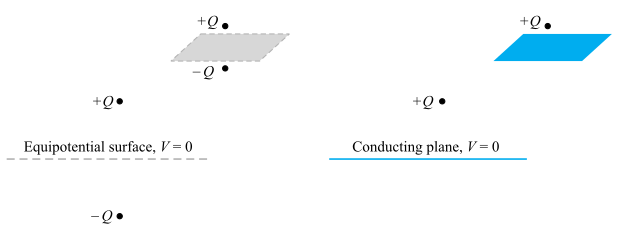
\includegraphics[scale=0.6]{img/image1.png}
	\caption{Méthode des images simple.}
	\label{fig:image1}
\end{figure}

Par linéarité, on peut répéter ce procédé encore et
encore comme illustré sur la figure \ref{fig:image2}. 

\begin{figure}[ht]
	\centering
	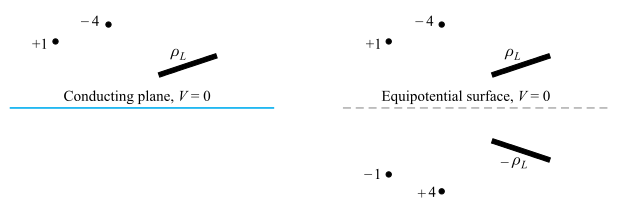
\includegraphics[scale=0.6]{img/image2.png}
	\caption{Méthode des images par linéarité.}
	\label{fig:image2}
\end{figure}

Dans plusieurs cas, le potentiel électrique du nouveau
système obtenu est plus simple à calculer puisqu'il ne
contient plus de plaque conductrice infinie avec une
densité de surface inconnue.

\subsection{Conducteur électrique parfait et conditions aux interfaces}
\begin{myprop}
Un conducteur électrique parfait possède les propriétés
suivantes :
\begin{enumerate}
	\item La densité de charge à l'intérieur du conducteur
	est nulle ;
	\item Toutes les charges se trouvent sur la surface du
	conducteur.
\end{enumerate}
En électrostatique (pas de courant), on a en plus
\begin{enumerate}
	\item Le champ électrique à l'intérieur du conducteur
	est nul ;
	\item Le champ tangentiel à la surface est nul.
\end{enumerate}
\end{myprop}

Mathématiquement, en appliquant \ref{eq:E-conservatif} sur
le chemin rectangulaire de la figure \ref{fig:conductor-boundary},
on trouve bien que la composante tangentielle de $\E$ est nulle
\begin{equation}
	\E \times \hat{n} \Big|_s = 0.
	\label{eq:cci-1}
\end{equation}
En appliquant \ref{eq:gauss} sur le cylindre de
la figure \ref{fig:conductor-boundary}, on trouve une
relation entre la composante normale à la surface et
la densité de charge du conducteur
\begin{equation}
	\D \cdot \hat{n} \Big|_s = \rho_s.
	\label{eq:cci-2}
\end{equation}
Dans ces deux équations, $\hat{n}$ est le vecteur unitaire
normal au conducteur et \textbf{sortant} du conducteur.

\begin{figure}[ht]
	\centering
	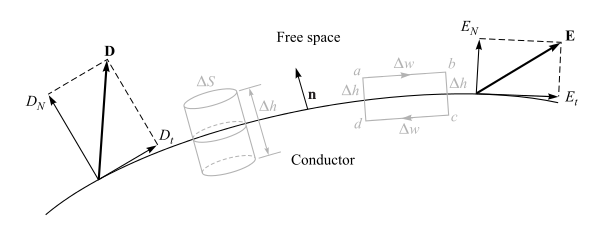
\includegraphics[scale=0.6]{img/conductor-boundary.png}
	\caption{Conditions limites pour un conducteur parfait.}
	\label{fig:conductor-boundary}
\end{figure}

\subsection{Nature des matériaux diélectriques}
Un matériau diélectrique dans un champ électrique peut être vu
comme un arrangement de minuscules dipôles électriques, chacun
composé d'une charge positive et d'une charge négative. Ces charges
ne sont pas libres et ne participent donc pas à la conduction,
ce sont des charges liées. Les diélectriques sont capables de
stocker de l'énergie. Ce stockage se fait via un décalage par
rapport à leur position d'équilibre des charges négatives et
positives qui constituent les minuscules dipôles.

Si on applique un champ électrique sur un matériau polarisable,
on arrive à une définition plus générale de $\D$ que ce qui
avait été fait précédemment
\begin{equation}
	\D = \perm_0\E + \P
\end{equation}
où $\P$ est la \emph{polarisation} du matériau. Pour les matériaux
dans lequels le champ $\E$ et la polarisation $\P$ sont
linéairement relié, on peut écrire
\begin{equation}
	\D = \perm_0\perm_r \E = \perm \E.
\end{equation}

\subsection{Diélectrique parfait et conditions aux interfaces}
En appliquant \ref{eq:E-conservatif} sur le chemin rectangulaire
de la figure \ref{fig:dielectric-boundary}, on trouve que le
le champ $\E$ tangentiel est continu aux interfaces
\begin{equation}
	(\E_1 - \E_2) \times \hat{n} = 0
\end{equation}
et donc automatiquement que le champ $\D$ tangentiel est
discontinu aux interfaces.

En appliquant \ref{eq:gauss} sur le cylindre de
la figure \ref{fig:dielectric-boundary}, on trouve
\begin{equation}
	(\D_1 - \D_2) \cdot \hat{n} = \rho_s
\end{equation}
où $\rho_s$ est la quantité de charge libre sur l'interface
(très souvent\footnote{\label{foot:rho}En fait il n'y a que deux cas pour
lequel la densité de charge dans un diélectrique (que ce soit
en surface ou en volume) n'est pas nulle. Le premier cas est celui
ou des charges ont été implantées dans le diélectrique isolant
(dopage). Le deuxième cas est celui où la conductivité est
variable.} 0).
Dans ces deux équations, $\hat{n}$ est le vecteur normal
à l'interface allant de la région 2 vers la région 1.

\begin{myrem}
On remarque que les conditions aux interfaces \ref{eq:cci-1}
et \ref{eq:cci-2} sont en fait des cas particuliers de
ces conditions pour $\E_2 = \D_2 = \vec{0}$.
\end{myrem}

\begin{figure}[ht]
	\centering
	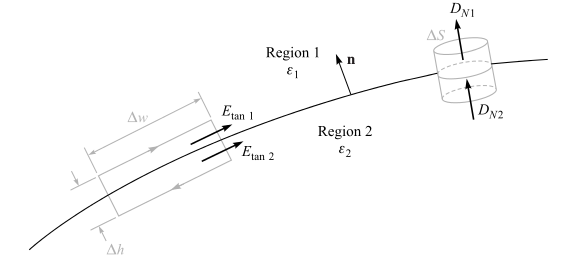
\includegraphics[scale=0.6]{img/dielectric-boundary.png}
	\caption{Conditions limites pour un diélectrique parfait.}
	\label{fig:dielectric-boundary}
\end{figure}

\section{Capacitance}
\begin{mydef}
La \textit{capacitance} de deux conducteurs portant
des charges opposés $Q$ et $-Q$ et dont
la différence potentiel est $V_0$ est définie comme
\begin{equation}
	C \eqdef \frac{Q}{V_0}.
	\u{\farad}
\end{equation}
\end{mydef}

En utilisant \ref{eq:gauss} et \ref{eq:potdef}, on
obtient
\begin{equation}
	C = \frac{\oint_S \perm\E \cdot \dif \vec{S}}{
	-\int_-^+ \E \cdot \dif \vec{L}}.
\end{equation}

\begin{myrem}
Lorsqu'on utilise cette dernière équation pour calculer
une capacitance, il faut faire attention. Lorsqu'on charge
une capacité, la somme totale des charges réparties dans
la capacité est nulle. Pour utiliser la dernière équation,
il ne faut donc considérer que les charges positives ou les
charges négatives (et si possible choisir le cas le plus
simple pour appliquer Gauss).
\end{myrem}

Pour une capacitance constitué de deux plaques
parallèles de surface $S$ et séparé par une distance
$d$, on a
\begin{equation}
	C = \perm\frac{S}{d}.
\end{equation}
L'énergie stockée dans cette capacitance est
donné par
\begin{equation}
	W_E = \frac{1}{2}CV^2 = \frac{1}{2}QV =
	\frac{1}{2}\frac{Q^2}{C}.
	\label{eq:energie-capa}
\end{equation}
\subsection{\'{E}quations de Laplace et de Poisson}
L'équation de Poisson permet d'obtenir un potentiel
en connaissant les valeurs de ce potentiels aux frontières
du problème. Elle s'obtient très facilement en utilisant
\ref{eq:gauss-dif}, \ref{eq:def-d} et \ref{eq:e-grad-v}
\[ \divn \D = \divn (\perm \E) = \perm\divn (-\gradn V) = \rho_v \]
ce qui peut finalement se réecrire
\begin{equation}
	\lap V = -\frac{\rho_v}{\perm}.
\end{equation}
Cette équation est valide pour une région homogène
dans laquelle $\perm$ est constant. Si $\rho_v = 0$,
l'équation de Poisson devient l'équation de Laplace
\begin{equation}
	\lap V = 0.
\end{equation}

\begin{mytheo}[Existence et unicité]
La solution d'une équation de Poisson dont les
conditions aux limites sont appropriées existe et
est unique.
\end{mytheo}

Ce théorème permet de justifier le fait que changer
le problème sans changer ses conditions aux limites
(grâce à la méthode des images par exemple) nous
fournit bien l'unique solution.

On peut résoudre une équation de Laplace par
séparation de variables (voir cours de mathématique 3).

% TODO: à faire relire
\newpage
\subsection{Travaux virtuels}
Le principe des travaux virtuels s'applique aux systèmes
isolés énergétiquement de l'extérieur, autrement dit 
aux systèmes dont l'énergie est conservée.

Imaginons que l'on veuille connaître la force $F_x$ s'exerçant sur
une plaque d'un condensateur isolé pour lequel $Q$ est constant.
On applique virtuellement une force de même norme (inconnue) et de
direction (inconnue) opposée et on va regarder comment le système
réagit afin de mesurer cette force.
On considère donc un déplacement infinitésimal d'une plaque d'un
condensateur. Si une force s'exerce sur cette plaque, cela
signifie qu'une certaine énergie peut-être récupérée lors
de ce déplacement (si on rapproche les plaques) ou doit être
fournie pour pemettre ce déplacement (si on éloigne les plaques).
\[ \Delta W_m = -\vec{F}_x \cdot \Delta\vec{x}. \]
Cette énergie retirée ou ajoutée au système doit être stockée
sous forme d'énergie électrique ou magnétique. Le changement
de géométrie du condensateur entraîne une différence
d'énergie. Si la charge $Q$ est constante, cette différence
est donnée par (en utilisant \ref{eq:energie-capa})
\[ \Delta W_e = \Delta\left(\frac{1}{2}\frac{Q^2}{C}\right). \]
%\[ \dif W_e = \fpart{}{C}\left(\frac{Q^2}{2C}\right) =
%\frac{Q^2}{2} \fpart{}{x}\left(\frac{1}{C(x)}\right). \]
On peut finalement écrire le bilan d'énergie
\[ \Delta W_e = \Delta W_m. \]
Si maintenant on relâche cette plaque, elle retournera à sa
position initiale en libérant (ou absorbant) toute
l'énergie $\Delta W_e$ stockée précédemment en subissant la
force $F_x$ inconnue que l'on veut déterminer.
Le bilan d'énergie nous permet donc d'écrire
\begin{align*} 
	-\vec{F}_x \cdot \Delta \vec{x} &= \Delta\left(\frac{1}{2}\frac{Q^2}{C}\right). \\
		& \text{On considère } Q \text{ constant ici.} \\
	F_x	&= -\frac{Q^2}{2}\Delta\left(\frac{1}{C}\right)\frac{1}{\Delta x} \\
		&= -\frac{Q^2}{2} \frac{\Delta\left(\frac{1}{C}\right)}{\Delta x} \\
		& \text{On fait maintenant tendre } \Delta x \text{ vers 0.} \\
		&= -\frac{Q^2}{2} \fpart{}{x}\left(\frac{1}{C(x)}\right).
\end{align*}
%\[ F_x = - \frac{Q^2}{2} \fpart{}{x}\left(\frac{1}{C(x)}\right). \]

De manière générale, on a pour un condensateur isolé
avec une charge $Q$ constante
\begin{center}
\textit{énergie mécanique fournie $=$ variation d'énergie du système}
\end{center}
et pour un condensateur raccordé à une source de
tension (pour maintenir $V$ constant)
\begin{center}
\textit{\textbf{énergie fournie par la batterie} $+$ énergie mécanique fournie
$=$ variation d'énergie du système}.
\end{center}

\part{Magnétostatique}
\section{Champ magnétique constant}
\subsection{Loi de Biot-Savart}
La loi de Biot-Savart en magnétostatique et l'analogue
de la loi de Coulomb en électrostatique.
\begin{mylaw}
Expérimentalement, on peut montrer qu'un champ magnétique
est produit par un courant continu $I$ circulant dans un élément
de longueur infinitésimal $\dl$ et vaut
\begin{equation}
	\vec{\dif H} = \frac{I\dl \times a_r}{4\pi R^2}.
	\u{\ampere\per\meter}
\end{equation}
Son sens est donné par la règle du tire-bouchon de la
main droite.
\end{mylaw}

On peut réecrire cette équation en utilisant la définition
de densité de courant
\begin{equation}
	\H = \int_{vol} \frac{\J \times \hat{a}_r}{4\pi R^2}\dV.
\end{equation}

\subsection{Loi d'ampère}
\begin{mylaw}
L'intégrale du champ $\H$ sur un chemin fermé est égale
au courant ``passant'' dans ce chemin fermé
\begin{equation}
	\oint \H \cdot \dl = \int_{in} \J \cdot \dS = I.
\end{equation}
\end{mylaw}
En utilisant le théorème de Stoke, on peut écrire cette
dernière équation sous forme différentielle\footnote{Une
interprétation très intuitive du rotationnel se trouve
à la page 199 du livre.}
\begin{equation}
	\rotn \H = \J.
	\label{eq:ampere-diff}
\end{equation}

\subsection{Flux magnétique et densité de flux magnétique}
\begin{mydef}
On définit la \textit{densité de flux magnétique} dans
le vide
\begin{equation}
	\B = \mu_0\H.
	\u{\tesla = \weber\per\meter\squared}
\end{equation}
\end{mydef}

\begin{mydef}
On définit maintenant le flux magnétique
\begin{equation}
	\Phi = \int_S \B \cdot \dS.
	\u{\weber}
\end{equation}
\end{mydef}

\begin{mylaw}[Loi de Gauss pour le champ magnétique]
La loi de Gauss pour le champ électrique stipulait
que le flux sortant d'une surface fermée devait provenir
d'une source (c'est à dire une charge) situé à l'intérieur
de cette surface fermée. Pour un champ magnétique, les lignes
de champs bouclent toujours sur elles-même, il n'y a pas
de monopôle magnétique
\begin{equation}
	\oint \B \cdot \dS = 0.
	\label{eq:gauss-magn}
\end{equation}
En utilisant le théorème de la divergence, on obtient
\begin{equation}
	\divn \B = 0.
	\label{eq:gauss-magn-dif}
\end{equation}
\end{mylaw}

\subsection{Potentiel scalaire et potentiel vecteur magnétique}
% Besoin de faire le potentiel scalaire?
\subsubsection{Potentiel vecteur}
En utilisant l'équation \ref{eq:gauss-magn-dif} et en
se rappellant que la divergence d'un rotationnel est toujours
nulle, on peut écrire
\begin{equation}
	\B = \rotn \A
\end{equation}
où est $\A~\si{[\weber\per\meter]}$ est-ce qu'on appelle
un \textit{potentiel vecteur magnétique}. Jusqu'ici on a
juste définit $\A$ comme un vecteur qui respecte les équations
obtenues précédemment. On peut déterminer $\A$ en
utilisant la loi de Biot-Savart, la définition de $\A$
et la définition de $\B$, on peut montrer que
\begin{equation}
	\A = \oint \frac{\mu_0 I\dl}{4\pi R}
\end{equation}
ce qui en comparaison avec l'équation \ref{eq:elec-pot}
ressemble bien à un potentiel. A nouveau, on peut utiliser
la définition de densité de courant pour réecrire cette
équation sous la forme
\begin{equation}
	\A = \int_{vol} \frac{\mu \J}{4\pi R}\dV.
\end{equation}

\section{Forces magnétiques, matériaux et inductance}
\subsection{Force de Lorentz}
\begin{equation}
	\vec{F} = Q(\E + \vec{v} \times \B)
\end{equation}

\subsection{Force sur un courant}
A partir de la force de Lorentz et en utilisant \ref{eq:convection}
et les définitions de densité de courant, on obtient
\begin{equation}
	\vec{\dif F} = I\dl \times \B.
	\label{eq:force-on-current}
\end{equation}

\subsection{Force et moment sur un circuit fermé}
La force totale sur une boucle fermée dans un champ uniforme
est toujours nulle. Ce n'est cependant pas le cas du
moment de force.
En utilisant \ref{eq:force-on-current} sur une boucle
de dimension infinitésimale, on trouve
\[ \dif\vec{T} = I\dS \times \B. \]
On définit le produit du courant dans la boucle et
du vecteur de surface de la boucle comme le
\textit{moment magnétique dipolaire}
\[ \dif\vec{m} = I\dS \]
et donc
\begin{equation}
	\dif\vec{T} = \dif\vec{m} \times \vec{B}.
\end{equation}

% TODO : nature des matériaux magnétiques +
% magnétisation et perméabilité

\subsection{Conditions limites magnétiques}
En appliquant la loi de Gauss pour les champs magnétiques
dans le cylindre de la figure \ref{fig:magnetic-boundary},
on obtient que les composantes normales de $\B$ sont
continues sur la frontière entre deux matériaux magnétiques
\begin{equation}
	\hat{n}\cdot(\B_1 - \B_2) = 0
\end{equation}
et donc automatiquement que le champ $\H$ normal est
discontinu.

En appliquant cette fois la loi d'Ampère sur le chemin
rectangulaire de la figure \ref{fig:magnetic-boundary},
on obtient
\begin{equation}
	\hat{n}\times(\H_1 - \H_2) = \vec{K}
\end{equation}
en admettant que la surface entre les deux milieux comporte
un courant surfacique de densité $\K$.

Comme pour les conditions limites entre deux matériaux
diélectrique, $\hat{n}$ est défini comme normale à l'interface
et allant de la région 2 vers la région 1.

\begin{figure}[ht]
	\centering
	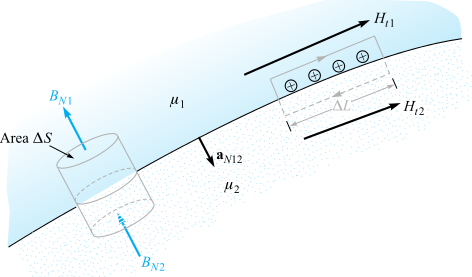
\includegraphics[scale=0.5]{img/magnetic-boundary.png}
	\caption{Conditions limites pour les matériaux magnétiques.}
	\label{fig:magnetic-boundary}
\end{figure}

\subsection{Circuits magnétiques}

\subsection{Energie potentielle magnétique}

\subsection{Inductance propre et mutuelle}
\begin{mydef}[Inductance propre]
On définit l'inductance comme le rapport entre le flux
total intercepté sur le courant
\begin{equation}
	L \eqdef \frac{\Phi_\text{tot}}{I}
	\u{\henry}.
\end{equation}
\end{mydef}

\begin{mydef}[Inductance mutuelle]
On définit l'inductance mutuelle
\begin{equation}
	M \eqdef \frac{\Phi_{2,1,tot}}{I_1} = \frac{\Phi_{1,2,tot}}{I_2}
\end{equation}
où $\Phi_{2,1}$ désigne le flux intercepté par 2 et produit par le
courant $I_1$. 
\end{mydef}

\section{Champs variables dans le temps}
\subsection{Loi de Faraday}
\begin{mylaw}
Expérimentalement, Faraday a pu montrer qu'un champ magnétique
variable dans le temps produit une force électromotrice
induite (emf ou $\EMF$) qui peut établir un courant sur un chemin fermé.
\begin{equation}
	\EMF = - \fdif{\Phi}{t}.
	\u{\volt}
\end{equation}
Le signe $-$ vient de la loi de Lenz qui stipule que la tension induite
s'oppose à la variation du flux.
\end{mylaw}

Par définition, l'emf est donnée par
\begin{equation}
	\EMF \eqdef \oint \E \cdot \dl
\end{equation}
et donc
\begin{equation}
	\EMF = \oint \E \cdot \dl = -\fdif{}{t} \int_S \B \cdot \dS.
\end{equation}
On peut réecrire cette dernière équation de manière différentielle
\begin{equation}
	\rotn \E = -\fpart{\B}{t}.
\end{equation}

\subsection{Courant de déplacement}
La loi d'Ampère sous forme différentielle est donnée par
l'équation \ref{eq:ampere-diff}. En prenant la divergence
de chaque côté de cette équation, on obtient
\begin{align*}
	\divn \rotn \H 	&= \divn \J \\
	0 				&= -\fpart{\rho_v}{t}
					\neq 0 \text{ en général.}
\end{align*}
Il y a donc une incohérence dans nos équations. Essayons
d'ajouter un terme $\vec{G}$ inconnu à l'équation
\ref{eq:ampere-diff} pour rendre notre modèle cohérent
\[ \rotn \H = \J + \vec{G}. \]
En reprenant la divergence de chaque côté, on obtient
\[ 0 = \divn \J + \divn \vec{G} \]
et donc
\[ \divn \vec{G} = \fpart{\rho_v}{t}. \]
En remplaçant $\rho_v$ par $\divn \D$, on a donc
\[ \divn \vec{G} = \fpart{\divn \D}{t} = \divn \fpart{\D}{t} \]
et par identification
\begin{equation*}
	\vec{G} = \fpart{\D}{t}.
\end{equation*}
$\vec{G}$ est appelé le courant de déplacement.

\subsection{Potentiels retardés}
%TODO quel est le lien entre tout ça et les potentiels retardés?
% (c'est dans la même section dans le livre mais j'ai dû mal à voir
% pourquoi, à éclaircir)
De la même manière, vérifions la cohérence de l'équation
\ref{eq:e-grad-v}. En prenant la rotationnel
de chaque côté de cette équation, on obtient
\begin{align*}
	\rotn (-\grad V)	&= \rotn \E \\
	0 				&= -\fpart{\B}{t}
					\neq 0 \text{ en général.}
\end{align*}
A nouveau, essayons d'ajouter un terme inconnu $\vec{N}$
à l'équation \ref{eq:e-grad-v} pour résoudre cette
incohérence.
\[ \E = -\grad V + \vec{N}. \]
En reprenant le rotationnel de chaque côté, on obtient
\[ \rotn \E = 0 + \rotn \vec{N}. \]
En utilisant la loi de Faraday, on a donc
\[ \rotn \vec{N} = -\fpart{\B}{t}. \]
Or, $\B = \rotn \A$
\[ \rotn \vec{N} = -\fpart{}{t}(\rotn \A) = -\rotn \fpart{\A}{t} \]
et donc par identification
\begin{equation*}
	\vec{N} = -\fpart{\A}{t}.
\end{equation*}

\section{Circuits magnétiques}
On peut résoudre un circuit magnétique de manière analogue
à un simple circuit éléctrique résistif. Pour cela,
définissons quelques nouveaux concepts.

\begin{mydef}
La force magnétomotrice $\MMF$ est donnée par
la loi d'Ampère
\begin{equation}
	\MMF \eqdef \oint \H \cdot \dl
	\u{\ampere}
	\label{eq:mmf}
\end{equation}
\end{mydef}

Un circuit magnétique étant en général constitué d'un
matériau magnétique dont une partie est entourée de
$N$ spires parcourues par un courant $I$, l'équation
\ref{eq:mmf} se réduit à
\begin{equation}
	\MMF = NI.
\end{equation}
Pour cette raison, la force magnétomotrice est parfois
donnée en ampères $\cdot$ tours.

\begin{mylaw}[Hopkinson]
La loi d'Hopkinson permet de relier le flux magnétique
$\Phi$ à la force électromotrice $\MMF$ au travers
d'une relation analogue à la loi d'Ohm
\begin{equation}
	\MMF = \Phi\relu
\end{equation}
où $\relu$ est la \emph{reluctance}.
\end{mylaw}
Bien que l'unité de la force magnétomotrice soit
l'ampère, son analogue en théorie des circuits est
donc bien la tension. Toujours par analogie à loi d'Ohm,
on voit que le flux $\Phi$ est analogue au
courant et bien sur que $\relu$ est analogue à la résistance.
\`{A} partir de toutes ces analogies, on peut
véritablement construire un circuit électrique équivalent
à un circuit magnétique.

\begin{mydef}
De la loi d'Hopkinson, on tire immédiatement la
définition de la reluctance
\begin{equation}
	\relu \eqdef \frac{\MMF}{\Phi} =
	\frac{\oint \H \cdot \dl}{\int \B \cdot \dS}.
	\u{\ampere\per\weber}
\end{equation}
\end{mydef}

Généralement, quand on résout un problème de circuit
magnétique, on fait les hypothèses suivantes :
\begin{enumerate}
	\item On néglige le \emph{champ de fuite}, ce qui
	revient à considérer l'air autour du circuit comme
	un isolant ;
	\item On néglige les effets de bords, ce qui nous
	permet de considérer que $\B$ est constant sur toute
	la section du matériau magnétique et donc d'utiliser
	des chemins d'intégration de longueur moyenne lorsqu'on
	utilise la loi d'Ampère mais surtout de grandement
	faciliter le calcul des flux.
\end{enumerate}

Armés de ces différentes hypothèses simplificatrices
et de la conservation du flux magnétique (équation
\ref{eq:gauss-magn}, la résolution d'un circuit
magnétique se fait généralement en 3 étapes :
\begin{enumerate}
	\item On décompose le circuit en différentes parties
	selon le milieu (matériau magnétique, vide, etc) ou selon
	la taille de la section (pour pouvoir décomposer
	l'intégrale sur un contour fermé de $\H$ dans la loi d'Hopkinson
	par une somme d'intégrale sur chaque partie). Comme on néglige
	les effets de bords, la reluctance devient simplement
	\begin{equation}
		\relu = \frac{1}{\mu} \int \frac{1}{S(x)} \dif x
	\end{equation}
	où $S(x)$ est la section du matériau magnétique.
	\item On obtient ainsi la reluctance totale en additionnant la
	contribution de chaque partie.
	\item On utilise la loi d'Hopkinson. 
\end{enumerate}

\part{Éléments de circuit}

TODO

\part{Ondes planes}

TODO: ondes planes, vecteur d'onde, vecteur de Poynting, etc.

\part{Lignes de transmission}

Une ligne de transmission est un conducteur électrique le long duquel un signal courant-tension
se propage. En pratique, on utilise le formalisme de ligne de transmission quand la fréquence est
grande (càd la longueur d'onde est petite ou du même ordre de grandeur que la taille du conducteur).
À basse fréquence, il n'y a pas besoin d'utiliser le formalisme de ligne de transmission car on peut
considérer le conducteur comme un conducteur parfait (courant et tension identiques aux deux
extrémités, éventuellement avec résistance série), ce qu'on fait souvent en théorie des circuits.

Concrètetement, on utilise le formalisme des lignes de transmission pour les câbles coaxiaux, lignes
planaires, circuits imprimés haute fréquence, tout câble qui relie à une antenne... et aussi pour
le réseau \SI{50}{Hz}.

Une ligne de transmission est typiquement une paire de fils, parcouru par des courants opposés.
On peut modéliser une partie infinitésimale de ligne de transmission comme sur la
figure~\ref{fig:telegraph-equation}: la ligne à une résistance série $R$, une inductance propre $L$,
des pertes par conduction entre les conducteurs $G$ et une capacitance entre les conducteurs $C$.

Dans ce cours, on travaille souvent dans le cas sans pertes, avec $R = 0$ et $G = 0$,
ce qui simplifie les expressions,
mais le formalisme reste le même (on a juste plus de complexes -;).

\section{Équations du télégraphe en régime harmonique}
\begin{figure}[ht]
	\centering
	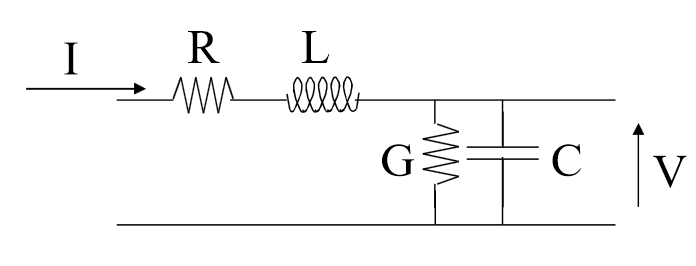
\includegraphics[scale=0.5]{img/telegraph-circuit.png}
	\caption{Schéma d'une ligne de transmission. Les éléments du circuits sont exprimés par unité de longueur.}
	\label{fig:telegraph-equation}
\end{figure}

La figure \ref{fig:telegraph-equation} représente une ligne de transmission tout à fait générale, dont les équations constitutives sont
\begin{equation}
	\fdif{V_s}{z} = -(R+j\omega L)I_s
\end{equation}
\begin{equation}
	\fdif{I_s}{z} = -(G+j\omega C)V_s
\end{equation}

\begin{myrem}
L'indice $_s$ fait référence au domaine de Laplace.
\end{myrem}

\subsection{Résolution du problème}
Les solutions des équations sont données par:

\begin{align}
	V_s &= V_0^+ e^{-\gamma z} + V_0^- e^{\gamma z} \\
	I_s Z_0 &= V_0^+ e^{-\gamma z} - V_0^- e^{\gamma z}
\end{align}

avec 

\begin{equation}
\begin{array}{|c|c|}
\hline
\text{Avec pertes} & \text{Sans pertes: $R=G=0$}\\
\hline
\displaystyle Z_0 =  \sqrt{\frac{R+j\omega L}{G+j\omega C}} &  \displaystyle Z_0 = \sqrt{\frac{L}{C}} \\
\displaystyle \gamma = \alpha + j\beta = \sqrt{(R+j\omega L)(G+j\omega C)} & \displaystyle \gamma = j\beta = j\omega \sqrt{LC}\\
\hline
\end{array}
\end{equation}
%TODO : ajouter des espaces verticaux

Remarquons également que 
\begin{equation}
\beta \eqdef \frac{\omega}{v_p}= \frac{2\pi}{\lambda}.
\end{equation}

\subsection{Quelques grandeurs caractéristiques}

\begin{mydef}
Le coefficient de réflexion en $z$ se définit, dans le cas sans pertes, comme:
\begin{equation}
\Gamma(z) \eqdef \frac{V_0^- e^{j\beta z}}{V_0^+ e^{-j\beta z}} = \frac{Z(z)-Z_0}{Z(z)+Z_0}.
\end{equation}
\end{mydef}

\paragraph{Impédance équivalente} L'impédance équivalente à une ligne terminée par une
charge d'impédance $Z_L$ vaut
\begin{equation}
Z_{in} = Z_0 \frac{Z_L\cos(\beta l)+jZ_0\sin(\beta l)}{Z_0\cos(\beta l) + j Z_L\sin(\beta l)}.
\label{eq:equiv-imp}
\end{equation}
Cette équation permet de calculer un circuit équivalent à un réseau de lignes de transmissions
et de charges.

\begin{myrem}
Si $Z_0 = Z_L$, alors l'onde réfléchie est nulle et
\begin{equation}
Z_{in} = Z_0.
\end{equation}
On parle alors de \emph{matching} d'impédance. Le but étant
en général de transmettre un maximum de puissance à la charge,
il est en général souhaitable de réduire l'onde réfléchie.
\end{myrem}

Notons quelques cas particuliers intéressants de l'équation
\ref{eq:equiv-imp} :
\begin{itemize}
	\item Si la longeur de la ligne est un multiple de $\lambda / 2$, on obtient
	\begin{equation}
		Z_{in}(l = m\lambda / 2) = Z_L.
	\end{equation}
	La ligne est alors en quelque sorte ``invisible'' et le circuit équivalent n'est
	constitué que de le charge.
	\item Si la longueur de la ligne est un multiple impair de $\lambda / 4$, on
	obtient cette fois
	\begin{equation}
		Z_{in}(l = (2m+1)\lambda / 4) = \frac{Z_0^2}{Z_L}.
	\end{equation}
	Grâce à cette propriété, on peut joindre deux lignes d'impédances caractéristiques
	$Z_{01} \neq Z_{03}$ tout en obtenant un coefficient de réflexion nul. En ajoutant
	une ligne d'impédance $Z_{02}$ entre ces deux
	lignes, on obtiendra une impédance d'entrée vue par la ligne 1 de
	\[ Z_{in} = \frac{Z_{02}^2}{Z_{03}}. \]
	Dès lors, en choisissant $Z_{02} = \sqrt{Z_{01}Z_{03}}$, on match l'impédance
	caractéristique de la ligne 1 avec l'impédance équivalente vue par celle-ci, et
	donc on évite la réflexion. On appelle ça un \textit{adaptateur quart d'onde}.
	\item Une ligne dont l'impédance de charge $Z_L$ est un court-circuit possède
	une impédance équivalente purement imaginaire $j Z_0 \tan \beta l$. 
	On peut mettre une telle ligne en
	parallèle avec une ligne dont on veut modifier l'impédance (typiquement pour annuler la
	partie imaginaire de l'impédance), et après utiliser une adaptation quart d'onde... on
	peut ainsi adapter une charge quelconque à un générateur donné.
\end{itemize}

\subsection{Abaque de Smith}

L'abaque de Smith permet de calculer graphiquement des impédances équivalentes. Il s'agit du disque
complexe des valeurs de $\Gamma$, sur lequel on a tracé les courbes iso-réelles et iso-imaginaires
pour l'impédance normalisée ($z = Z_L/Z_0$) correspondant au $\Gamma$.

Se déplacer le long d'une ligne de transmission revient donc à tourner le point autour du centre
($\Gamma = 0$ ou $z=1$).

On peut également utiliser directement l'abaque avec des admittances ($y=Y_L/Y_0$), il suffit de
lire les axes pour prendre les bons signes.

\section{Transitoires}

Ici, plus question de phaseurs:
\begin{align}
	\fpart{v}{z} &= -Ri-l\fpart{i}{t} \\
	\fpart{i}{z} &= -Gv-C\fpart{v}{t}
\end{align}

Dans le cas sans pertes, il reste
\begin{align*}
	\fpart{v}{z} &= -l\fpart{i}{t} \\
	\fpart{i}{z} &= -C\fpart{v}{t} \\
\end{align*}

On trouve \[c = \frac{1}{\sqrt{LC}}\]
et
\begin{align*}
	v(z, t) &= f_+(t-z/c) + f_-(t+z/c) \\
	Z_c i(z, t) &= f_+(t-z/c) - f_-(t+z/c) \\
\end{align*}

avec \[Z_c = \sqrt{\frac{L}{C}}\].

On a donc deux ondes progressives, une dans chaque sens.

On va donc analyser ce qu'il se passe dans le temps pour différents signaux de source
(typiquement, impulsions ou échelons).

\subsection{Générateur}

Si on a une ligne (d'impédance $Z_c$ et de longueur $l$) connectée à un générateur
d'impédance $R_s$, et une tension au générateur ($V_s(t) = 0$ si $t < 0$), on sait
que pour $t<0$, $v(z, t) = 0$ et $i(z, t) = 0$.

Donc $f_+(t-z/c) = f_-(t+z/c) = 0$. Du coup, en $z=0$, $f_-(t+z/c) = 0$ pour tout $t < l/c$.
Du coup, $V_s(t) - R_s i(t) = v(0, t) = f_+(t)$ et $R_c i(0, t) = f_+(t)$. On en
déduit \[f_+(t) = \frac{R_c}{R_s+Z_c} V_s(t).\]
La ligne se comporte donc au début comme une impédance, et on a un diviseur résistif à la
sortie du générateur.

\subsection{Charge}

On montre que à l'extrémité de la ligne, avec une charge $Z_L$, il y a une réflexion:
\[f_- = \frac{Z_L - Z_c}{Z_L + Z_c}\]
le coefficient de réflexion est le même que dans le cas harmonique.

Pour traiter le cas de multiple lignes, il ne faut pas faire d'impédances équivalentes
(ça n'a pas de sens: le signal ne peut pas "savoir" ce qu'il y a au bout de la ligne),
il suffit de considérer la propagation du signal dans le temps en prenant chaque fois
en compte les coefficients de réflexion (un diagramme adéquat aidera à n'oublier aucun
signal).
%TODO ajouter diagramme réflexions transitoire

Dans le cas où le signal n'est pas une impulsion mais un échelon (ou autre chose), on
fait la même chose et à l'arrivée on a non pas une impulsion mais le signal de départ
(avec une autre amplitude, évidemment), et plusieurs signaux peuvent s'additionner en
amplitude.

\part{Guides d'ondes}

\section{Ondes TEM, TM et TE}
\subsection{Considérations générales}
On distingue 3 types de propagation d'onde.
\begin{itemize}
\item les ondes TEM (\textit{Transverse Electro-Magnetic}), dont les deux
composantes $\E$ et $\H$ sont perpendiculaires à la direction de propagation
(voir figure \ref{fig:tem}).
\item les ondes TE (ou TM), dont seule la composante $\E$ (ou $\H$) est
perpendiculaire à la direction de propagation (voir figure \ref{fig:te-and-tm}).
La composante non perpendiculaire se déplace alors sous forme d'un "zig-zag",
en se réfléchissant successivement sur la plaque supérieur et la plaque inférieure
du conducteur. Pour qu'une de ces onde puisse se propager, il faut que toutes
les ondes qui se propagent "vers le haut" (c'est vrai aussi pour les ondes
qui se propagent "vers le bas") soient en phase, ce qui n'est possible que
pour des valeurs discrètes d'\textbf{angle d'incidence} $\theta$. L'existence
de cet angle dépend de la fréquence. Il existe dont une \textbf{fréquence de coupure}
pour chaque type de mode, en-dessous de laquelle l'onde TM ou TE ne se propagera
pas.

\begin{figure}[ht]
	\centering
	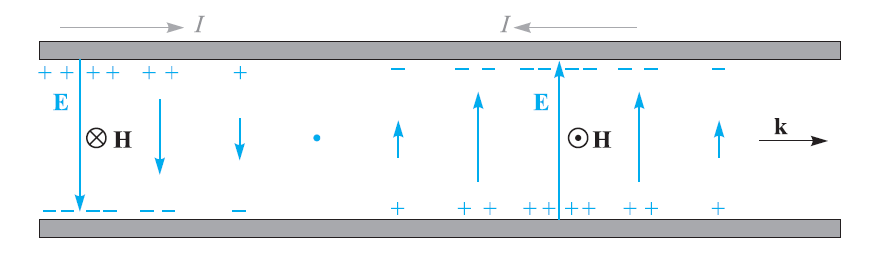
\includegraphics[scale=0.5]{img/tem.png}
	\caption{Représentation d'une TEM dans une ligne de transmission.}
	\label{fig:tem}
\end{figure}
\begin{figure}[ht]
	\centering
	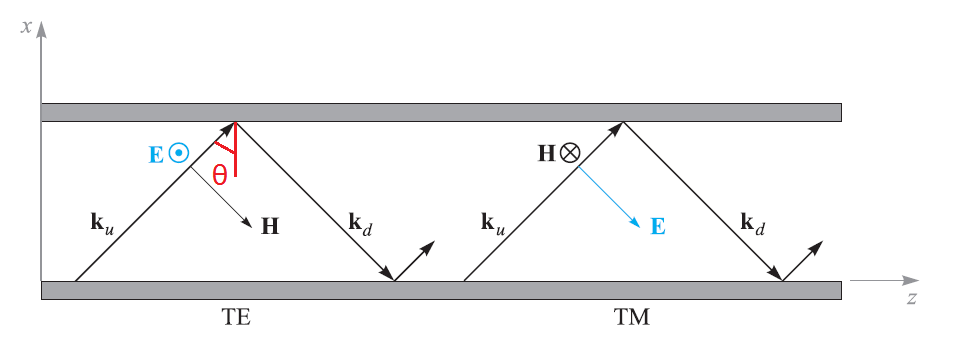
\includegraphics[scale=0.5]{img/te-and-tm.png}
	\caption{Représentation des modes TE et TM dans un guide d'onde à plaques parallèles.}
	\label{fig:te-and-tm}
\end{figure}
\end{itemize}

\begin{myrem}
Lorsque l'on étudie les lignes de transmission, on ne s'intéresse fondamentalement
qu'à la propagation d'ondes TEM. Dans le cadre de l'étude des guides d'ondes, on
s'intéresse également aux ondes TE et TM.
\end{myrem}
\begin{myrem}
Les ondes TEM n'ont pas de fréquence de coupure, et sont donc supportées
à toutes les fréquences. Cependant, certains types de guides d'ondes ne
sont tout simplement pas capable de les propager, compte tenu de leur design
(c'est le cas des guides d'ondes rectangulaires).
\end{myrem}
\begin{myrem}
Les modes TE et TM ne sont pas uniques. En réalité, il existe une grande
variété de solutions. De manière plus générale, on note ainsi $TE_{mn}$ et
$TM_{mn}$, où les indices $m$ et $n$ font référence à un type de solution
bien précis (voir figure \ref{fig:te_mn}).
\begin{figure}[ht]
	\centering
	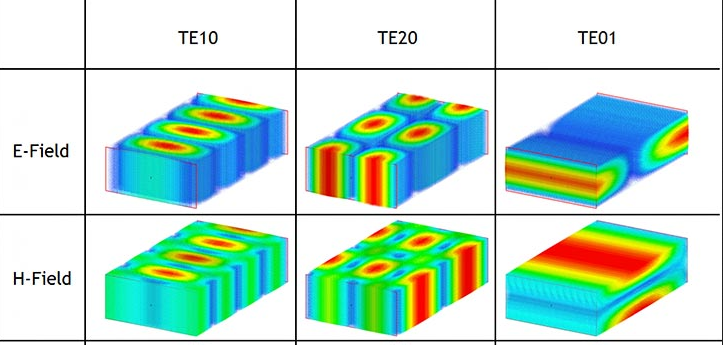
\includegraphics[scale=0.5]{img/te_mn.png}
	\caption{Différent modes $TE_{mn}$ dans un guide d'ondes rectangulaire.}
	\label{fig:te_mn}
\end{figure}
\end{myrem}
\begin{mydef}
(rappel de physique 3) Les grandeurs caractéristiques d'une onde
electromagnétique sont:
\begin{equation}
\omega = 2\pi f \hspace{1cm} f = \frac{1}{T} \hspace{1cm} k = \frac{2\pi}{\lambda} \hspace{1cm} v = \lambda f = \frac{\omega}{k}= \sqrt{\frac{1}{\epsilon \mu}}
\end{equation}
Plus particulièrement, on peut en extraire
\begin{equation}
k = \omega \sqrt{\epsilon \mu}.
\label{eq:rappelphysique3}
\end{equation}
\end{mydef}

\subsection{Résolution des équations de Maxwell et fréquence de coupure}
Lorsque l'on applique les équations de Mawell en régime harmonique,
et qu'on cherche les solutions stationnaires, on tombe sur les équations
de Helmoltz
\begin{equation}
\frac{\partial^2 E_z}{\partial^2 x} + \frac{\partial^2 E_z}{\partial^2 y} + p E_z = 0
\end{equation}

\begin{equation}
\frac{\partial^2 H_z}{\partial^2 x} + \frac{\partial^2 H_z}{\partial^2 y} + p E_z = 0
\end{equation}

Dans ces équations, $p$ a été définit d'après la relation
\begin{equation}
p^2 = \gamma ^2 + k^2
\label{eq:valpropres}
\end{equation}

Où $k$ représente le vecteur d'onde et où $\gamma$ vient de l'hypothèse
selon laquelle les champs suivant la direction $\vec{z}$ sont constant
à un facteur $e^{-\gamma z}$. Ainsi, le champs décroit exponentiellement
lorsque $\gamma$ est réel (les modes ne se propagent pas), alors que
l'exponentielle devient un simple terme de phase lorsque $\gamma$ est
imaginaire.

Soit $\omega_c$ la pulsation de coupure. La valeur de $\gamma$ est donnée par:
\begin{equation}
\gamma^2 = \left\{
\begin{array}{ll}
\alpha ^2 > 0 & \text{si } \omega \textless \omega_c \\
(j\beta ) ^2 < 0 & \text{si } \omega \textgreater \omega_c
\end{array}
\right.
\end{equation}

En combinant avec les équations \ref{eq:rappelphysique3} et \ref{eq:valpropres},
on obtient
\begin{equation}
\begin{array}{l}
\alpha = \sqrt{p^2 - \omega ^2 \epsilon \mu}\\
\beta = \sqrt{\omega ^2 \epsilon \mu - p^2}
\end{array}
\end{equation}

\begin{myprop}
La fréquence de coupure est la fréquence au-dessus de laquelle $\gamma$ est
imaginaire et en-dessous de laquelle $\gamma$ est réel. Il faut donc imposer
$\alpha = 0 \ (= \beta) $, et on obtient donc 
\begin{equation}
\omega_{cmn}^2 = \frac{p_{mn}^2}{\epsilon \mu}
\end{equation}
où $m$ et $n$ font référence au mode. L'expression de $p_{mn}$ varie selon le type de guide d'onde utilisé.
\end{myprop}

\section{Guides d'ondes rectangulaire}

Les équations des champs $\E$ et $\H$ pour les modes TE et TM sont données
dans le formulaire et ne sont pas reprises ici. 

\end{document}
